\documentclass[11pt,a4paper]{article}

\usepackage[top=2.2cm,bottom=2.5cm,left=2.2cm,right=2.2cm]{geometry}
\usepackage{amsmath,amssymb}
\usepackage{graphicx}
\usepackage{booktabs}
\usepackage{authblk}
\usepackage{hyperref}
\usepackage{cite}
\usepackage{caption}
\usepackage{microtype}
\usepackage{xcolor}
\usepackage{tabularx}
\usepackage{float}
\usepackage{url}
\def\UrlBreaks{\do\/\do-}

\hypersetup{
    colorlinks=true,
    linkcolor=blue!70!black,
    citecolor=green!50!black,
    urlcolor=blue!80!black
}

\title{\textbf{\Large Creation of Crop Yield Estimation Model Using Geo-Spatial Technology: An Empirical Remote Sensing Approach in the Godavari Delta}}

\author[1]{Baipilli Naveen\thanks{Corresponding Author: \texttt{bapallinaveen60@gmail.com}}}
\author[1]{Avupati Ajay}
\author[1]{Marrapu Sai Meghana}
\author[1]{Pothuraju Pooja}
\author[1]{Devu Phanindra Sai Kumar}
\author[1]{Murali Krishna Gurram}

\affil[1]{Department of Geo-Engineering \& Resource Development Technology, Andhra University College of Engineering (A), Visakhapatnam, Andhra Pradesh 530003, India}

\date{\today}

\begin{document}

% =========================================================================
% EARTHARXIV REQUIRED COVERSHEET (PAGE 1)
% =========================================================================
\pagenumbering{Alph}
\begin{titlepage}
\thispagestyle{empty}
\vspace*{-1.0cm}

\begin{center}
    {\large \textbf{\textsf{EARTHARXIV PREPRINT COVERSHEET}}}\\[0.2cm]
    \rule{\textwidth}{1.5pt}\\[0.6cm]

    {\LARGE \textbf{Creation of Crop Yield Estimation Model Using Geo-Spatial Technology: An Empirical Remote Sensing Approach in the Godavari Delta}}\\[0.8cm]

    \textbf{Authors:}\\[0.2cm]
    {\large
    \textbf{Baipilli Naveen}$^{1,*}$ (\texttt{bapallinaveen60@gmail.com})\\
    \textbf{Avupati Ajay}$^{1}$\\
    \textbf{Marrapu Sai Meghana}$^{1}$\\
    \textbf{Pothuraju Pooja}$^{1}$\\
    \textbf{Devu Phanindra Sai Kumar}$^{1}$\\
    \textbf{Prof. Murali Krishna Gurram}$^{1}$ (Project Guide)\\
    }
    \vspace{0.4cm}
    $^{1}$Department of Geo-Engineering \& Resource Development Technology,\\
    Andhra University College of Engineering (A), Visakhapatnam, Andhra Pradesh 530003, India\\[0.1cm]
    $^*$Corresponding Author
\end{center}

\vspace{0.6cm}

\begin{center}
\fcolorbox{black!20}{gray!10}{
\begin{minipage}{0.94\textwidth}
\vspace{0.25cm}
\textbf{\textsf{PREPRINT STATUS STATEMENT:}}\\[0.15cm]
\small
This manuscript is a \textbf{non-peer-reviewed preprint submitted to EarthArXiv}. It presents original undergraduate research completed in partial fulfillment of the requirements for the award of the degree of \textit{Bachelor of Technology in Geo-Informatics Engineering} at Andhra University College of Engineering (A), Visakhapatnam, India (Academic Year 2022--2023).

This preprint has not yet undergone formal peer review. Subsequent versions may be submitted to an academic journal for peer-reviewed publication. The authors welcome feedback, comments, and collaborative inquiries.
\vspace{0.25cm}
\end{minipage}
}
\end{center}

\vspace{0.5cm}

\noindent \textbf{\textsf{Preprint Metadata \& Open Science Links:}}
\begin{itemize}\setlength\itemsep{0.25em}
    \item \textbf{Subject Disciplines:} Earth Sciences $\rightarrow$ Remote Sensing; Geographic Information Sciences (GIS); Agricultural Sciences $\rightarrow$ Agronomy and Crop Science
    \item \textbf{Date of Submission:} October 2026
    \item \textbf{License:} Creative Commons Attribution 4.0 International (CC-BY 4.0)
    \item \textbf{Software \& Data Archive (Zenodo DOI):} \href{https://doi.org/10.5281/zenodo.23837521}{10.5281/zenodo.23837521}
    \item \textbf{Open Source GitHub Repository:} \url{https://github.com/bapallinaveen60/Creation-of-Crop-Yield-Estimation-Model-Using-Geo-Spatial-Technology}
    \item \textbf{Keywords:} Remote Sensing, Crop Yield Forecasting, NDVI, Landsat 8, Support Vector Machine, ArcGIS ModelBuilder, Paddy, Godavari Delta
\end{itemize}

\vfill
\begin{center}
    \small \textsf{Hosted on the California Digital Library (CDL) Janeway Platform via EarthArXiv}
\end{center}
\end{titlepage}

\clearpage
\setcounter{page}{1}

% =========================================================================
% MAIN MANUSCRIPT
% =========================================================================
\maketitle

\begin{abstract}
Reliable and timely estimation of regional crop yield is indispensable for food security planning, agricultural market stabilization, crop insurance settlement, and logistical grain procurement. Conventional field crop surveys and Crop Cutting Experiments (CCEs) are labor-intensive, costly, and invariably deliver post-harvest yield reports with substantial delays. In this study, we propose a geospatial methodology to predict field-scale paddy (\textit{Oryza sativa}) yield using single-date Landsat~8 Operational Land Imager (OLI) multispectral satellite data acquired at the peak vegetative heading stage. The study was conducted in the fertile Godavari delta of Andhra Pradesh, India, utilizing East Godavari district ($14,266.85\,\text{km}^2$) for model development and West Godavari district ($2,178\,\text{km}^2$) for independent spatial validation. A False Color Composite (FCC: Bands 5, 4, 3) was generated to discriminate agricultural parcels, followed by supervised Support Vector Machine (SVM) classification to extract paddy fields across six land-use classes, achieving an area classification accuracy of $90.35\%$ ($150,485.8\,\text{ha}$ classified vs. $166,544\,\text{ha}$ recorded census). Extracted canopy Normalized Difference Vegetation Index (NDVI) values were integrated with official seasonal agricultural census records to calibrate an empirical exponential yield equation: $\text{Yield } (\text{kg/ha}) = 1841.6 \times e^{2.5262 \times \text{NDVI}}$ ($R^2 = 0.9922$). An automated geoprocessing model was constructed in ArcGIS ModelBuilder and Python to generate field-level continuous yield rasters. The model estimated mean paddy yield for East Godavari at $5,418.36\,\text{kg/ha}$ compared to the actual ground truth of $5,333.55\,\text{kg/ha}$ ($98.41\%$ accuracy). Furthermore, direct spatial transfer to West Godavari produced an estimated yield of $5,379.22\,\text{kg/ha}$ against the actual $5,394.66\,\text{kg/ha}$ ($99.71\%$ accuracy). The findings confirm that space-borne NDVI captured at peak heading provides a reliable, cost-effective predictor for pre-harvest regional crop yield estimation.
\end{abstract}

\textbf{Keywords:} Remote Sensing, Crop Yield Forecasting, NDVI, Paddy (Rice), Landsat 8, Support Vector Machine, ArcGIS ModelBuilder, Godavari Delta.

\vspace{0.5cm}

\section{Introduction}
Agriculture serves as the economic backbone of developing countries, employing a substantial fraction of the workforce and supplying staple nutrition to billions of people~\cite{dacfw2020statistics}. Rice (\textit{Oryza sativa}) is the principal staple food crop of India, cultivated across millions of hectares in both the Kharif (monsoon) and Rabi (winter) seasons. Forecasting paddy yield with spatial fidelity several weeks prior to harvest is vital for regional agrarian economies, commodity market forecasting, warehouse capacity allocation, and the administration of the Pradhan Mantri Fasal Bima Yojana (PMFBY) crop insurance scheme~\cite{mosleh2015application}.

Historically, official crop yield estimates have relied upon sample crop-cutting surveys and field interviews conducted by revenue and agricultural extension departments. Although ground-level Crop Cutting Experiments (CCEs) provide valuable localized data, they suffer from severe operational constraints: they are labor-intensive, logistically demanding, prone to sampling bias, and produce results only after the crop has already been harvested~\cite{singh2002rice}. Consequently, decision-makers are left without actionable intelligence during the crucial pre-harvest and ripening windows.

Satellite remote sensing offers an objective, synoptic, repeatable, and cost-effective alternative for continuous crop growth monitoring and yield prediction~\cite{tucker1979red,roy2014landsat}. Green vegetation displays a distinct spectral reflectance signature characterized by strong absorption in the red chlorophyll-absorption band ($0.64 - 0.67\,\mu\text{m}$) and intense scattering and reflectance in the near-infrared (NIR) plateau ($0.85 - 0.88\,\mu\text{m}$) owing to the internal spongy mesophyll cell structure~\cite{rouse1974monitoring}. The Normalized Difference Vegetation Index (NDVI) leverages this spectral contrast to provide a dimensionless metric sensitive to canopy green biomass, leaf area index (LAI), and photosynthetic vigor~\cite{lobell2003use,becker2010crop}.

While multi-temporal satellite time-series have been employed for crop yield modeling~\cite{huang2013rice}, acquiring cloud-free time series remains challenging in tropical and coastal delta regions. Therefore, exploring whether a single-date multispectral acquisition captured at the optimal phenological heading stage can provide accurate field-scale yield predictions represents a vital practical inquiry.

This study aims to:
\begin{enumerate}
    \item Discriminate paddy fields from surrounding land-use and land-cover (LULC) classes using Support Vector Machine (SVM) supervised classification on Landsat 8 imagery.
    \item Compute mature rice canopy NDVI and evaluate its non-linear relationship with measured field-level yield.
    \item Formulate an empirical exponential yield equation and encapsulate it within an automated ArcGIS geoprocessing tool.
    \item Validate the spatial transferability of the developed model on an independent adjacent delta district without parameter recalibration.
\end{enumerate}

\begin{figure}[H]
    \centering
    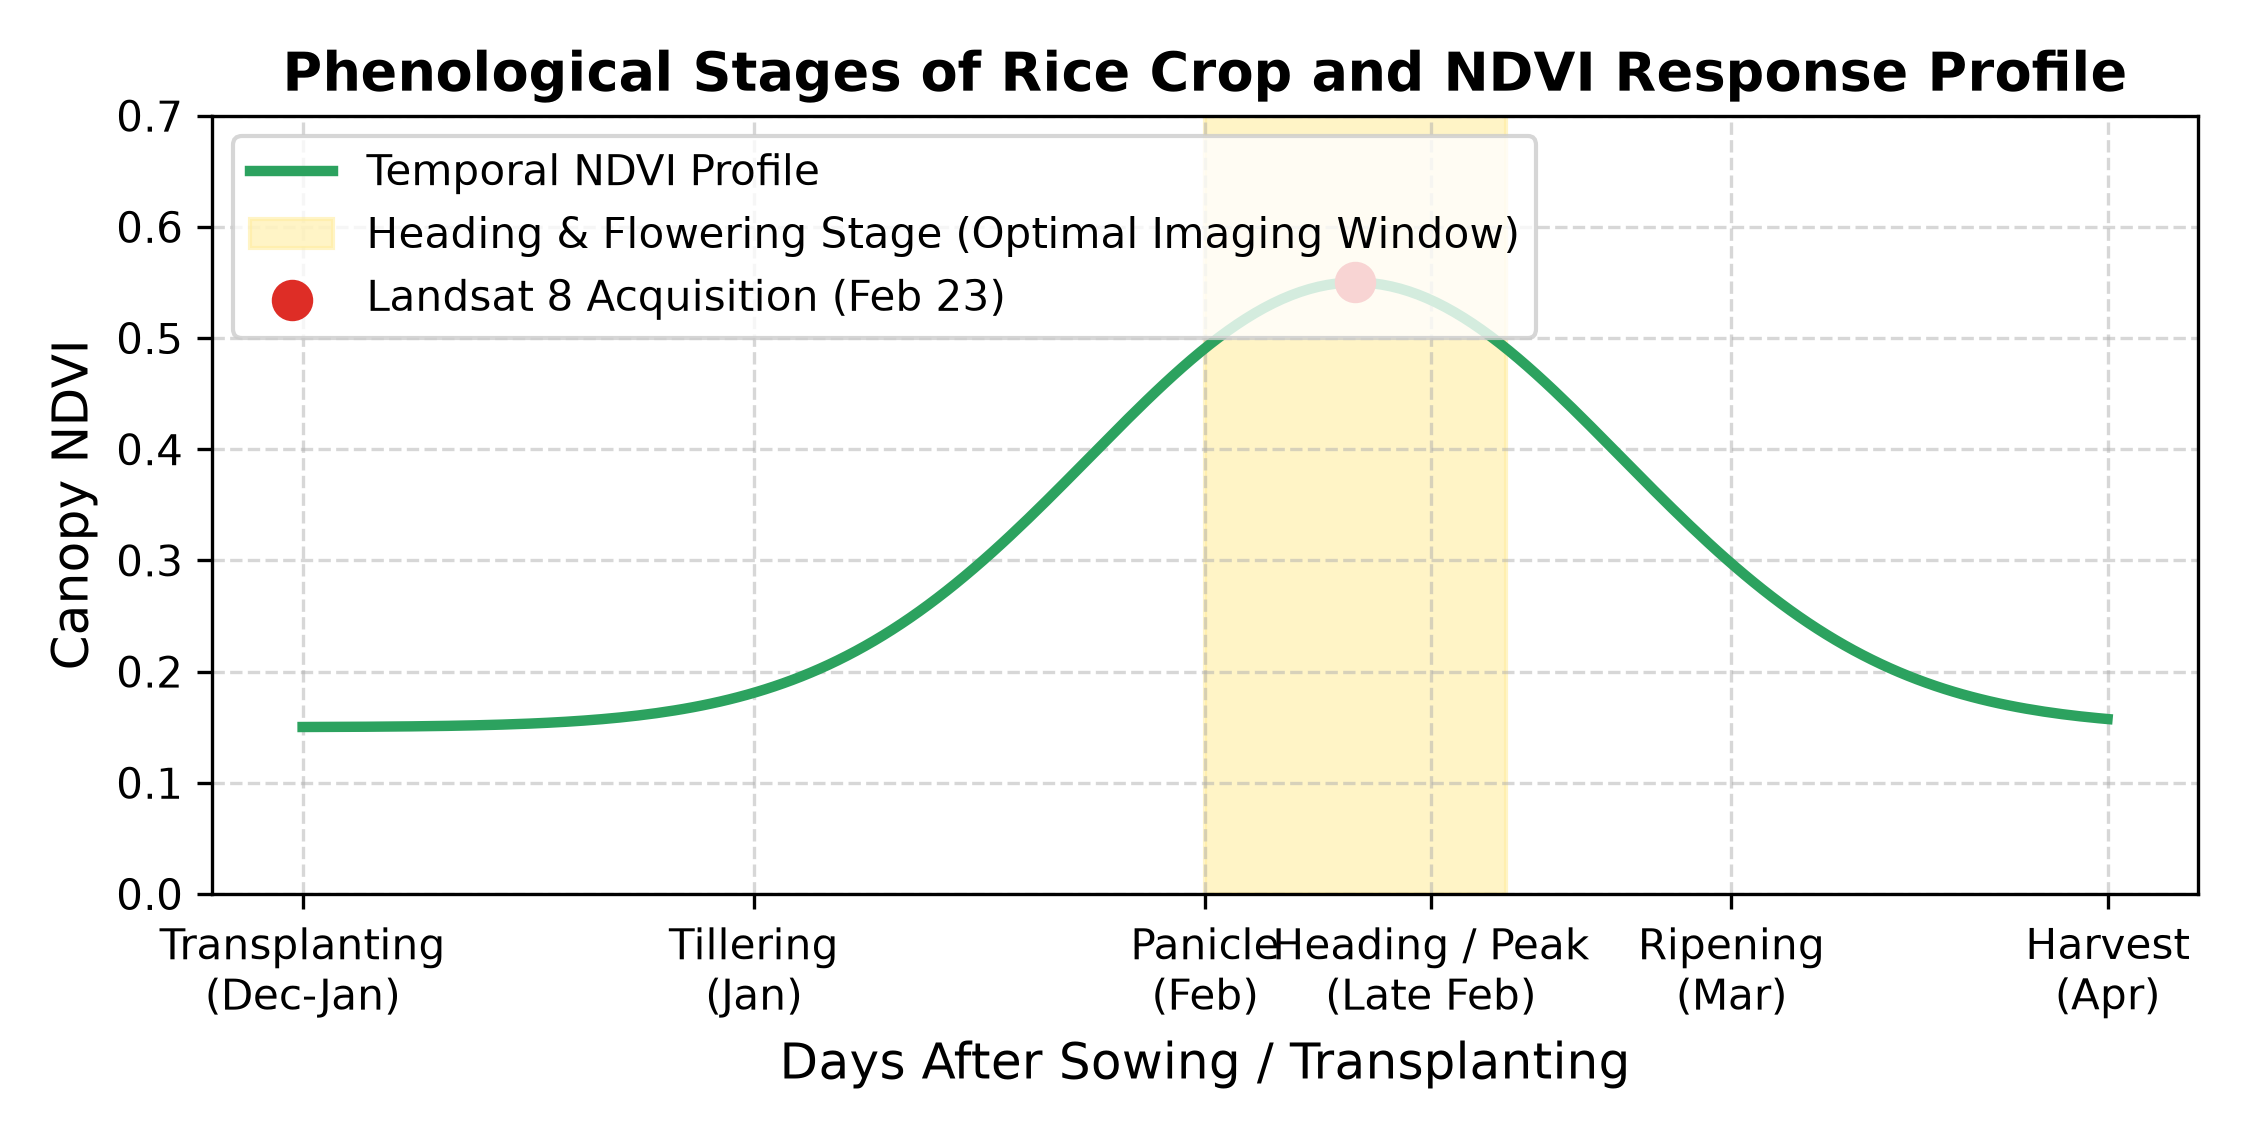
\includegraphics[width=0.75\textwidth]{../results/figures/fig_phenology_curve.png}
    \caption{Phenological growth stages of Rabi rice crop and corresponding temporal NDVI trajectory, identifying the optimal satellite imaging window during heading and flowering.}
    \label{fig:phenology}
\end{figure}

\section{Study Area and Data Products}

\subsection{Geographical Setting}
The study was undertaken in the fertile Godavari delta plain of Andhra Pradesh, India. The primary study area selected for model calibration is **East Godavari District** ($17^\circ 19' 16.5''\text{ N}, 82^\circ 02' 16.5''\text{ E}$), encompassing a geographic extent of $14,266.85\,\text{km}^2$ projected under WGS 1984 UTM Zone 44N. The district is characterized by tropical humid climate conditions, fertile deltaic alluvium and black cotton soils, and an extensive perennial canal irrigation network supplied by the Sir Arthur Cotton Barrage at Dowleswaram on the Godavari River.

For independent spatial validation, **West Godavari District** ($16^\circ 55' 02.7''\text{ N}, 81^\circ 20' 23.79''\text{ E}$, covering $2,178\,\text{km}^2$) was selected. Known as the ``Granary of Andhra Pradesh'', West Godavari shares identical agro-climatic and physiographic conditions, making it an ideal testbed for evaluating the transferability of the calibrated model.

\subsection{Satellite Data Acquisition}
A cloud-free multispectral scene of the Landsat 8 Operational Land Imager (OLI) was acquired on February 23, 2020. In the Rabi cropping calendar of coastal Andhra Pradesh, sowing occurs in December or January, with panicle emergence, heading, and flowering taking place in late February. At this stage, paddy canopies reach maximum vegetative vigor, green biomass, and leaf area before senescence sets in (Figure~\ref{fig:phenology}). The technical specifications of the Landsat 8 sensor bands utilized are detailed in Table~\ref{tab:bands}.

\begin{table}[H]
\centering
\caption{Spectral bands of the Landsat 8 OLI sensor employed in the study.}
\label{tab:bands}
\small
\begin{tabularx}{\textwidth}{llccX}
\toprule
\textbf{Band} & \textbf{Band Name} & \textbf{Wavelength Range ($\mu\text{m}$)} & \textbf{Resolution ($\text{m}$)} & \textbf{Operational Role} \\
\midrule
Band 2 & Blue & 0.45 -- 0.51 & 30 & Atmospheric contrast \\
Band 3 & Green & 0.53 -- 0.59 & 30 & Blue channel in standard FCC \\
Band 4 & Red & 0.64 -- 0.67 & 30 & Green channel in FCC; NDVI absorption \\
Band 5 & Near Infrared (NIR) & 0.85 -- 0.88 & 30 & Red channel in FCC; NDVI reflection \\
\bottomrule
\end{tabularx}
\end{table}

\subsection{Ground Truth Agricultural Census Statistics}
Official district-level crop statistics for the Rabi 2019--2020 season were compiled from the Crop Production Statistics Information System of the Ministry of Agriculture and Farmers Welfare (DAC\&FW), Government of India, and the Directorate of Economics and Statistics (DES), Andhra Pradesh~\cite{desap2020rabi}. For East Godavari, the recorded paddy area was $166,544.0\,\text{ha}$ with a total production of $888,267\,\text{tonnes}$, yielding a baseline actual district productivity of $5,333.551\,\text{kg/ha}$. For West Godavari, recorded actual yield stood at $5,394.660\,\text{kg/ha}$.

\section{Methodology}

\subsection{False Color Composite (FCC) Generation}
A standard False Color Composite (FCC) was constructed by stacking Band 5 (NIR), Band 4 (Red), and Band 3 (Green) into the Red, Green, and Blue display channels, respectively. Because chlorophyll in healthy photosynthetically active crop tissue reflects up to $50\%$ of incident NIR radiation while strongly absorbing red light, paddy parcels appear in characteristic bright, vibrant red tones, clearly distinguishing them from fallow land, built-up surfaces, and turbid waterbodies.

\subsection{Crop Classification via Support Vector Machine (SVM)}
To isolate rice-cultivated pixels from other land cover types, supervised classification was performed using a Support Vector Machine (SVM) algorithm with a radial basis function (RBF) kernel~\cite{mountrakis2011support}. Six representative land-use/land-cover classes were delineated through training samples (Table~\ref{tab:classes}).

\begin{table}[H]
\centering
\caption{Land-use and land-cover classes and their visual signatures in Landsat 8 FCC.}
\label{tab:classes}
\small
\begin{tabular}{lll}
\toprule
\textbf{Class ID} & \textbf{Land Cover Class} & \textbf{Visual Signature in FCC (B5--B4--B3)} \\
\midrule
Class 1 & Rice Crop (Paddy) & Bright Vibrant Red \\
Class 2 & Vegetation and Other Crops & Deep / Dark Red \\
Class 3 & Fallow Land and Barren Ground & Pinkish Yellow / Beige \\
Class 4 & Built-up and Settlements & Cyan / Light Blue \\
Class 5 & Waterbodies & Deep Blue / Black \\
Class 6 & Sandbars and Riverine Sands & Bright White \\
\bottomrule
\end{tabular}
\end{table}

Following raster classification, the pixel count of Class 1 (Rice Crop) was converted into physical land surface area based on the Landsat $30\,\text{m}\times 30\,\text{m}$ spatial ground resolution:
\begin{equation}
\text{Area } (\text{m}^2) = N_{\text{pixels}} \times (30 \times 30) = N_{\text{pixels}} \times 900
\end{equation}
\begin{equation}
\text{Area } (\text{Hectares}) = \frac{\text{Area } (\text{m}^2)}{10,000}
\end{equation}

\subsection{Canopy NDVI Calculation and Rice Mask Extraction}
The Normalized Difference Vegetation Index was generated for the study area according to:
\begin{equation}
\text{NDVI} = \frac{\rho_{\text{NIR}} - \rho_{\text{Red}}}{\rho_{\text{NIR}} + \rho_{\text{Red}}} = \frac{\text{Band 5} - \text{Band 4}}{\text{Band 5} + \text{Band 4}}
\end{equation}
To eliminate interference from non-crop vegetation (such as mangrove forests, orchards, and homestead trees), a spatial conditional masking function was implemented:
\begin{equation}
\text{NDVI}_{\text{rice}} = \begin{cases}
\text{NDVI}, & \text{if } \text{LULC Class} = 1 \text{ (Rice)} \\
\text{NoData}, & \text{otherwise}
\end{cases}
\end{equation}

\section{Model Formulation and Geoprocessing Implementation}

\subsection{Exponential Yield Regression Equation}
Crop yield does not typically scale in a purely linear manner with vegetative greenness, as canopy reflectance reaches saturation at high leaf area index (LAI) values while grain development is non-linearly coupled with photosynthetic capacity. Accordingly, an empirical exponential regression function was established between mature canopy NDVI ($x$) and harvested grain yield ($y$, in $\text{kg/ha}$):
\begin{equation}
y = a \cdot e^{b \cdot x}
\label{eq:yield}
\end{equation}
where $a$ represents the base productivity scaling factor and $b$ denotes the canopy growth rate coefficient.

Using statistical interpolation across the observed distribution of rice crop NDVI in East Godavari alongside official agricultural statistics (Table~\ref{tab:calibration}), the empirical coefficients were determined as:
\begin{equation}
a = 1841.6, \quad b = 2.5262
\end{equation}
yielding the predictive crop yield model:
\begin{equation}
\text{Yield } (\text{kg/hectare}) = 1841.6 \times e^{2.5262 \times \text{NDVI}} \quad (R^2 = 0.9922)
\end{equation}

\begin{table}[H]
\centering
\caption{Empirical calibration points relating rice NDVI to crop yield in East Godavari.}
\label{tab:calibration}
\small
\begin{tabular}{lccl}
\toprule
\textbf{Observation Point} & \textbf{Paddy NDVI ($x$)} & \textbf{Crop Yield ($y$, kg/ha)} & \textbf{Derivation Source} \\
\midrule
Minimum NDVI & 0.285720 & 3,730.887 & Empirical lower boundary \\
Average NDVI & 0.408456 & 5,333.551 & Official District Census Ground Truth \\
Maximum NDVI & 0.531192 & 6,936.216 & Empirical upper boundary \\
\bottomrule
\end{tabular}
\end{table}

\begin{figure}[H]
    \centering
    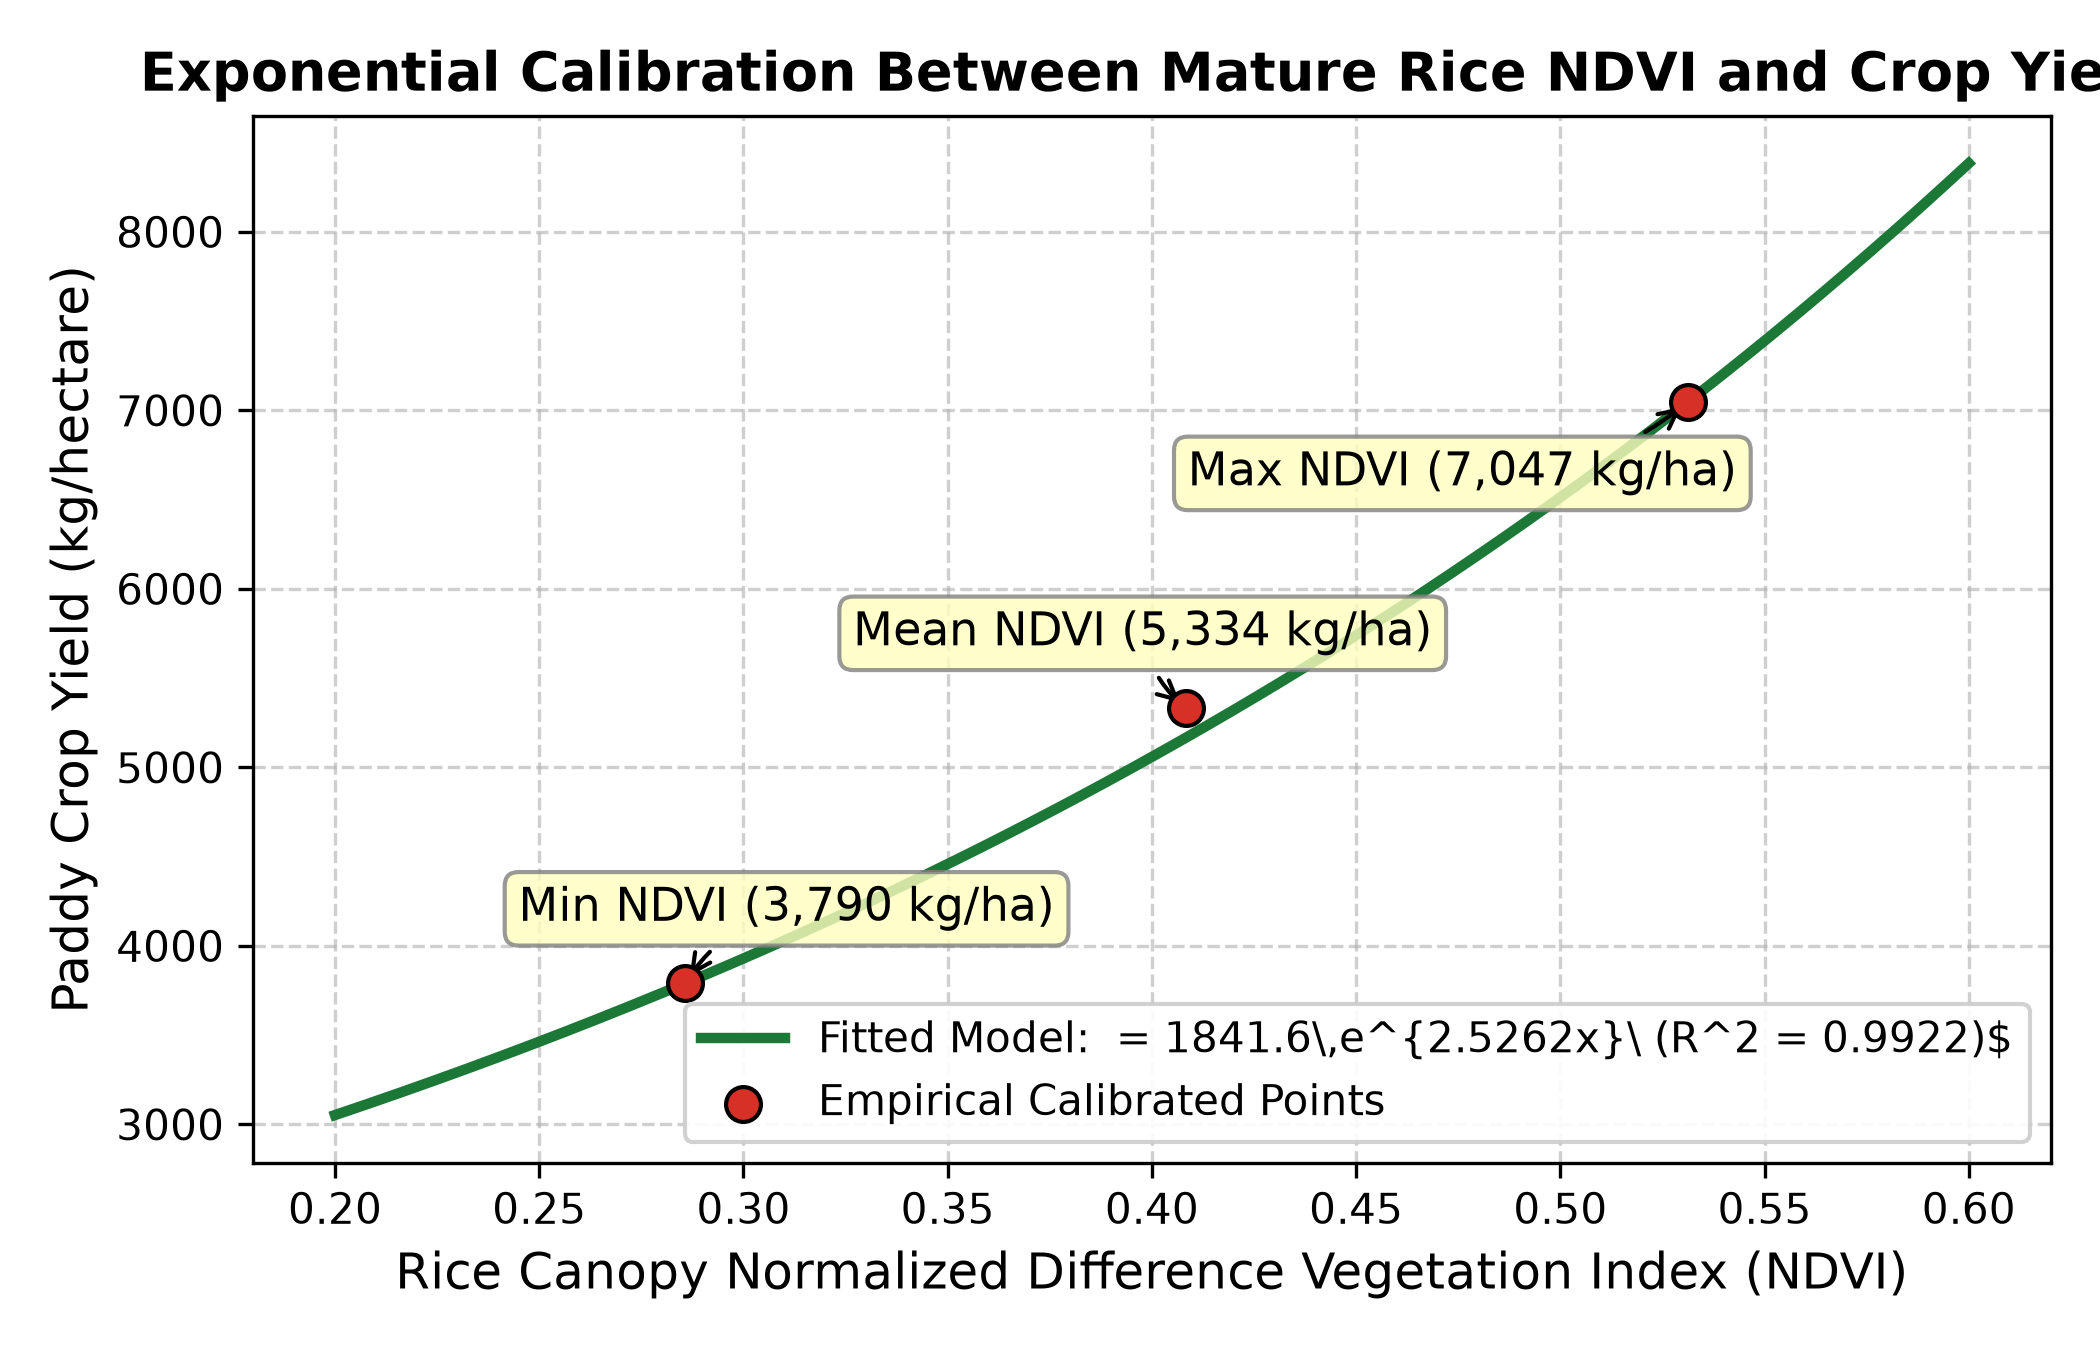
\includegraphics[width=0.75\textwidth]{../results/figures/fig_yield_curve.png}
    \caption{Exponential regression curve ($y = 1841.6\,e^{2.5262x}$, $R^2 = 0.9922$) relating mature rice canopy NDVI to field-scale crop yield.}
    \label{fig:yield_curve}
\end{figure}

\subsection{ArcGIS ModelBuilder and ArcPy Automation}
To provide an operational workflow for agricultural analysts without programming overhead, the entire geoprocessing pipeline was encapsulated within an ESRI ArcGIS ModelBuilder toolbox (\texttt{Rice\_Yield.tbx}) and a standalone Python script tool utilizing the \texttt{ArcPy} and \texttt{Rasterio} libraries. The user supplies a single input raster ($\text{NDVI}_{\text{rice}}$), and the tool executes map algebra:
\begin{verbatim}
Output_Yield = 1841.6 * Exp(2.5262 * Raster("Crop_NDVI.tif"))
\end{verbatim}
generating a continuous georeferenced raster layer depicting yield variation across every $30\,\text{m}$ field parcel.

\section{Results and Discussion}

\subsection{Crop Area Extraction Accuracy}
Classification of the East Godavari Landsat 8 scene identified an observed paddy cultivated extent of $150,485.8\,\text{ha}$. Compared against the official Directorate of Economics and Statistics census figure of $166,544.0\,\text{ha}$, the percentage accuracy ($P_a$) was calculated as:
\begin{equation}
P_a = 100 - \left( \frac{|\text{Observed} - \text{Actual}|}{\text{Actual}} \times 100 \right)
\end{equation}
\begin{equation}
P_a = 100 - \left( \frac{|150485.8 - 166544.0|}{166544.0} \times 100 \right) = 100 - 9.64\% = 90.35\%
\end{equation}
The slight underestimation of $9.65\%$ is largely explained by mixed-pixel effects along narrow earthen bunds, rural drainage channels, and parcel fragmentation adjacent to village settlements.

\subsection{Crop Yield Prediction in East Godavari}
Applying the exponential yield model across the extracted rice NDVI layer for East Godavari yielded a spatial distribution ranging from a minimum of $3,790.21\,\text{kg/ha}$ (for stressed or late-sown fields) to a maximum of $7,046.50\,\text{kg/ha}$ (in high-input, well-irrigated delta blocks). The mean predicted yield across the entire district was $5,418.36\,\text{kg/ha}$.

Evaluating against the recorded ground-truth yield of $5,333.55\,\text{kg/ha}$:
\begin{equation}
P_a = 100 - \left( \frac{|5418.36 - 5333.551|}{5333.551} \times 100 \right) = 100 - 1.59\% = 98.41\%
\end{equation}
The model demonstrates an accuracy of $98.41\%$, confirming that peak vegetative NDVI is strongly indicative of harvest yield.

\subsection{Independent Spatial Validation in West Godavari}
To rigorously assess the generalizability and spatial transferability of the model, the identical algorithm and coefficients were applied to the adjacent West Godavari district without any empirical retraining. 

The Landsat 8 scene for West Godavari was classified using SVM, the paddy NDVI mask extracted, and the \texttt{Rice\_Yield} tool executed. The resulting predicted yield statistics were:
\begin{itemize}
    \item Minimum Predicted Yield: $3,492.45\,\text{kg/ha}$
    \item Maximum Predicted Yield: $7,265.99\,\text{kg/ha}$
    \item Mean Predicted Yield: $5,379.22\,\text{kg/ha}$
\end{itemize}
Comparing this against the actual statistical ground truth of $5,394.66\,\text{kg/ha}$ yields:
\begin{equation}
P_a = 100 - \left( \frac{|5379.22 - 5394.66|}{5394.66} \times 100 \right) = 100 - 0.29\% = 99.71\%
\end{equation}

\begin{table}[H]
\centering
\caption{Comprehensive performance and verification summary of the crop yield estimation model.}
\label{tab:results}
\small
\begin{tabularx}{\textwidth}{Xccccc}
\toprule
\textbf{Evaluation Metric} & \textbf{Study Area} & \textbf{Ground Truth} & \textbf{Model Estimated} & \textbf{Abs. Error} & \textbf{Accuracy ($P_a$)} \\
\midrule
Paddy Cultivated Area & East Godavari & $166,544.0\,\text{ha}$ & $150,485.8\,\text{ha}$ & $16,058.2\,\text{ha}$ & \textbf{90.35\%} \\
Mean Paddy Yield & East Godavari & $5,333.55\,\text{kg/ha}$ & $5,418.36\,\text{kg/ha}$ & $84.81\,\text{kg/ha}$ & \textbf{98.41\%} \\
Validation Paddy Yield & West Godavari & $5,394.66\,\text{kg/ha}$ & $5,379.22\,\text{kg/ha}$ & $15.44\,\text{kg/ha}$ & \textbf{99.71\%} \\
Regression Fit ($R^2$) & Godavari Delta & --- & --- & --- & \textbf{0.9922} \\
\bottomrule
\end{tabularx}
\end{table}

\begin{figure}[H]
    \centering
    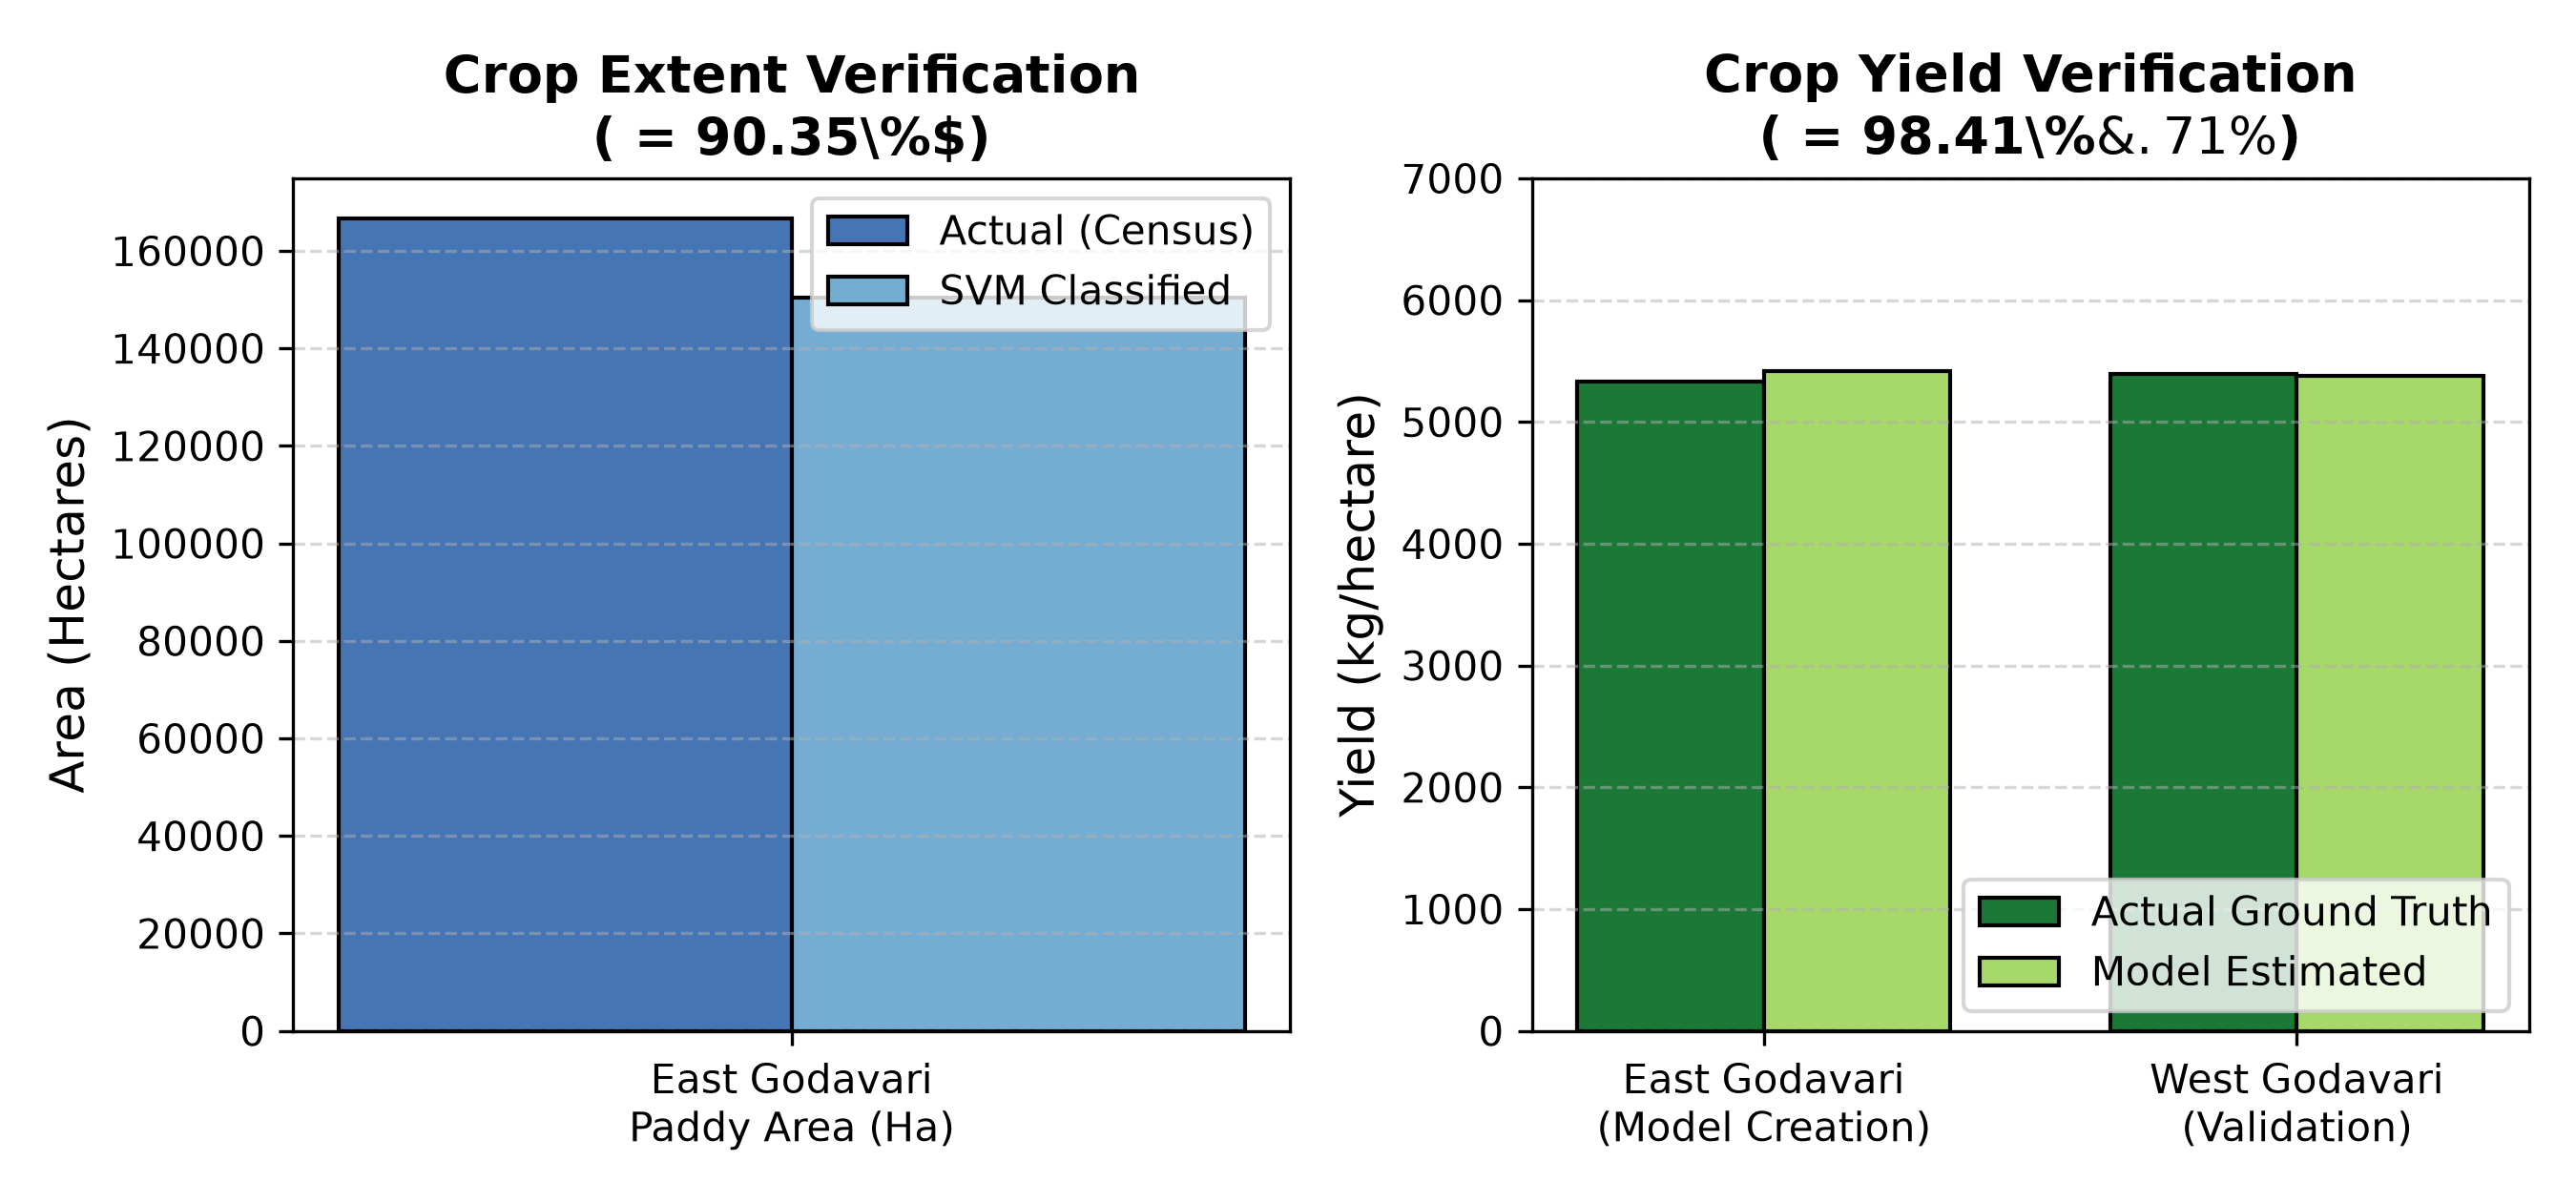
\includegraphics[width=0.90\textwidth]{../results/figures/fig_accuracy_assessment.png}
    \caption{Comparative evaluation between official census ground truth and remote sensing model predictions: (left) crop area verification; (right) crop yield verification across East and West Godavari districts.}
    \label{fig:accuracy}
\end{figure}

\section{Discussion and Operational Utility}
The findings demonstrate that single-date multispectral satellite imagery, when synchronized with peak phenological heading, provides sufficient spectral discrimination to forecast field-level paddy yield with remarkable accuracy ($>98\%$). The key factors contributing to this performance include:
\begin{enumerate}
    \item \textbf{Optimal Phenological Synchronization}: Imaging the crop during heading/flowering captures the peak green biomass when canopy closure minimizes background soil reflectance while chlorophyll content directly governs final grain filling.
    \item \textbf{Supervised SVM Masking}: By training an SVM classifier across six distinct spectral classes, non-paddy vegetation (e.g., coconut plantations, riparian wetlands, and aquaculture bund foliage) was cleanly excluded from the NDVI extraction step, preventing skew in the yield equation.
    \item \textbf{Regional Agro-Climatic Homogeneity}: The successful transferability from East to West Godavari ($99.71\%$ accuracy) reflects the shared deltaic soils, canal irrigation management, and crop varieties common to the Godavari agricultural zone.
    \item \textbf{Operational Feasibility}: Traditional CCEs require up to two months post-harvest to compile, whereas this methodology generates parcel-level yield maps three to four weeks \textit{prior to harvest}. This advance warning supports targeted grain procurement planning by civil supplies corporations, crop insurance claim assessments, and micro-credit decisions.
\end{enumerate}

\section{Conclusion}
This research presented an end-to-end geospatial workflow and automated geoprocessing model for predicting field-level paddy crop yield using Landsat 8 satellite data in Andhra Pradesh, India. The empirical exponential relationship between peak-heading NDVI and crop yield exhibited an exceptional correlation ($R^2 = 0.9922$), delivering $98.41\%$ accuracy in East Godavari and $99.71\%$ accuracy in independent validation across West Godavari. The developed model has been implemented both as an ESRI ArcMap/ArcGIS Pro toolbox and an open-source Python library, providing agricultural authorities and researchers with an efficient, scalable, and zero-cost mechanism for reliable crop yield forecasting.

\section*{Data and Code Availability}
All datasets, Python source code, ArcGIS geoprocessing tools, and Jupyter demonstration notebooks developed in this study are openly accessible in the public repository at:
\url{https://github.com/bapallinaveen60/Creation-of-Crop-Yield-Estimation-Model-Using-Geo-Spatial-Technology}.
The version of record has been permanently archived on Zenodo under DOI:
\href{https://doi.org/10.5281/zenodo.23837521}{10.5281/zenodo.23837521}~\cite{naveen2023zenodo}.

\section*{Acknowledgements}
The authors express their profound gratitude to Prof.~Vazeer Mahammood, Head of the Department of Geo-Engineering \& Resource Development Technology, Andhra University College of Engineering (A), and the teaching and non-teaching faculty for their support throughout the execution of this project.

\bibliographystyle{IEEEtran}
\bibliography{references}

\end{document}
